% !TeX spellcheck = en_US
\documentclass[]{article}

\usepackage{amsmath, xparse}

\usepackage{graphicx}


 \usepackage{easyReview}


%opening
\title{\comment{3D Voxel Grid Based Path Planning for Robotic Manipulators using Matrix Multiplication Technique}{Alternatives:\\ - Efficient distance calculation / Efficient repulsive field calculation technique \\   - Matrix Multiplication-Driven Repulsive Fields for 3D Voxel-Based Robotic Manipulator Path Planning \\ - Robotic Manipulator Path Planning Optimization Using Matrix-Derived Repulsive Fields Based on 3D Voxel Grid}}

\author{Jakob Baumgartner, Gregor Klančar}

\begin{document}
	
\maketitle

\comment{}{for keywords use the SEO algorithm to find which terms are popular}

\begin{abstract}

\end{abstract}

\section{Introduction}


\subsection{Motion Planning}

% PREDSTAVITEV REDUNDANCE

Kinematic redundancy~\cite{siciliano1990kinematic, siciliano2016springer} enables a manipulator to follow a predefined task space trajectory using the endeffector (EE), while simultaneously, optimising for an additional task with the remaining movement capacity without impacting the trajectory adherence. This is possible because the robot's degrees of freedom (DOF) go beyond what is required to perform the primary task. Consequently, the robot can adopt different joint configurations optimised according to the secondary task while performing the primary task. Common secondary tasks~\cite{siciliano2010robot} include avoiding singularities, optimising the manipulability measure, minimising joint torques and avoiding obstacles in the operating space.

% PREDSTAVITEV PRISTOPOV PLANIRANJA POTI V ROBOTIKI
The task of finding the joint trajectories of a manipulator is called motion planning~\cite{IDEASLab2023}. It consists of finding a sequence of joint configurations for a robot so that the robot can move along this path from its initial configuration to the goal configuration without colliding with itself, static obstacles or other agents in the environment. In addition to collision avoidance, motion planning for manipulators can optionally take into account various constraints, such as position, velocity, acceleration or jerk constraints for the joint angle or end effector, precision of the end effector with respect to position and orientation, stability of the manipulator, avoidance of singularities, or any number of other criteria.

There are numerous methods for planning manipulator movements~\cite{c51, c52}, they can rougly be seperated into global and local approaches. Global, sampling-based, methods such as PRM~\cite{vsvestka1997motion}, RRT*~\cite{lavalle1998rapidly, karaman2010incremental}, RRT-Connect~\cite{kuffner2000rrt}, Informerd RRT*~\cite{gammell2014informed}, BIT*~\cite{gammell2015batch} and others offer a globally optimal solution based on a global search in configuration space. However, the generated trajectories are not always smooth or optimal, and the performance of the methods may be insufficient for real-time operation.

%Global planning methods are typically more comprehensive, aiming to find a globally optimal trajectory for the manipulator. These methods often involve mapping out the entire path before movement begins, taking into account the known environment, which usually includes static obstacles. However, the downside of global planning methods is their computational intensity, which often renders them too slow for real-time applications. This limitation is particularly pronounced in dynamic or unpredictable environments where conditions change rapidly and require quick responses. Examples of global planning methods include graph-based algorithms like A* and Dijkstra's algorithm, which are known for their effectiveness in pathfinding but also for their computational demands [(Lavalle, 2006)].

%Sampling-based methods such as PRM, RRT, RRT*, RRT-Connect, Informerd RRT*, BIT* and others offer a solution based on a global search in configuration space. However, the generated trajectories are not always smooth or optimal, and the performance of the methods may be insufficient for real-time operation. 

\remove{Recently, a number of learning-based methods using data-driven techniques have been proposed to improve or accelerate the functionality of sampling-based methods. }

\remove{Trajectory optimisation methods such as CHOMP, STOMP and TrajOpt, on the other hand, use optimization to improve an initial seed trajectory. Consequently, the optimality of the solution is highly dependent on this initial trajectory. Nevertheless, these methods are capable of generating smooth trajectories, and although they can be too computationally intensive for high DOF dynamic real-time environments, they are generally effective in finding constrained motion plans. }

Local motion planning approaches employ optimization techniques, two common ones are inverse kinematics~\cite{c29,c38}, that is based on finding a least squares solution of the manipulator joint velocities, and quadratic programming (QP)~\cite{c21,c22, haviland2021neo, c23}.  Both methods are fast, suitable for real-time applications in dynamic environments and provide smooth solutions. However, since they do not plan further than one step ahead, they tend to get stuck in local minima. Therefore, they are often combined with a higher-level planner, for global static environment based \replace{motion}{path} planning, while local optimisation takes dynamic environment changes into account. In the following text we will focus on inverse kinematics based approaches.

\subsection{Kinematic Obstacle Avoidance}

\remove{Different control schemes have been proposed. Acceleration-based control excels in precise handling of motion changes, velocity-based control offers consistent and smooth movement, while force and torque-based control provides direct control over joint forces for robust physical interactions. (CITATIONS in COMMENT BELLOW)}
%\remove{Different control schemes have been proposed~\cite{c24}. Acceleration-based control excels in precise handling of motion changes, velocity-based control offers consistent and smooth movement, while force and torque-based control~\cite{c25, c26, c27, c28, c31} provides direct control over joint forces for robust physical interactions.}

% ----

%In our work we use velocity control strategy for obstacle avoidance using the manipulator. naša primarna naloga premik vrha robota - end efektorja (EE) v želeno pozo, to je točko in orientacijo v prostoru naloge. Naša sekundarna naloga se tako izvaja v preostalem prostoru gibanja sklepov redundance robota (DOF, DOR). ??? je predlagal razširitev jakobijeve matrike end-efektorja z dodatno matriko transformacije izogibne hitrosti iz kartzezičnega prostora v prostor sklepov. Če nalogi nista popolnoma neodvisni ena od druge, in njune sklepne hitrosti niso medsebojno ortagonalne, lahko to pripelje do medsebojnega oviranja izbajanja nalog. Zato je ??? predlagal uporabo transformacijo hitrosti sekundarne naloge v  ničelnega prostora hitrosti primarne nalgoe, to je v prostor ortagonalnih hitrosti. Posledično izvajanje sekundarne naloge ne vpliva neposredno v izvajanje primarne naloge, gledano le v enem trenutku izvajanja. 
%
%Različni razisklovalci so se lotili problema kinematičnega izogibanja na različne načine, kot je opisano v \cite{c30, c39}. 
%
%Colbaugh in Glass  1989 \cite{c31, c32} sta se problema lotila v dveh korakih. V prvem koraku sta izračunala trajektorijo vrha robota, v drugem pa sta uporabila optimizacijo za izboljšanje dinamičnega odziva robota med izvajanjem trajektorije in za druge naloge, kot so izogibanje ovir.  
%
%Sciavicco and Siciliano \cite{c34, c35} and Egeland~\cite{c36} independetly introduced the concept ot task-space augmentation. It was later revisited by searji~\cite{c37}. The Solution is to stack the remaining rows in Jacobian with secondary task Jacobian into square matrix, that returns only one solution.
%
%Macijewski in Klein (Maciejewski & Klein, 1985) \cite{c29}, Nakamura in Hanafusa 1987 \cite{c38} predstavijo koncept prioritete nalog in ničelnega prostora za izogibanje, pri čemer se sekundarna naloga lahko giblje le s hitrostmi, ki ne vplivajo neposredno na gibanje primarne naloge. pri čemer sta izogibne sklepne hitrosti izračunala funkcijo najmanjše razdalje med točko na manipulatorju in točko izogibanja / objekta / ovire.  
%
%Omenjeni pristopi se ne osredotočajo na okolje, tega pogosto prikažejo kot geometrijske primitive in nato razdaljo izračunajo kot razdaljo med primitivom in premicami, ki opisujejo manipulator. 
%
%Khatib \cite{c33} proposes the concept of Artificial Potential Field. Polje sestavljata odbojna komponenta, ki end effektor odbija od ovir, ki so predstavljene kot geometrijski primitivi in privlačna komponenta, ki manipulator privlači proti cilju. 
%
%
%

Various researchers have adopted different approaches to kinematic avoidance, as detailed in~\cite{c30, c39}.

Colbaugh and Glass (1989)~\cite{c31, c32} tackled this problem in a two-step process. Initially, they calculated the robot's end-effector trajectory. Subsequently, they used optimization to enhance the robot's dynamic response during trajectory execution and for tasks like obstacle avoidance.

Sciavicco and Siciliano~\cite{c34, c35}, as well as Egeland~\cite{c36}, independently introduced the concept of task-space augmentation, later revisited by Searji~\cite{c37}. This method involves extending the primary task Jacobian with the secondary task Jacobian into a square matrix, yielding a singular solution.

Maciejewski and Klein (1985)~\cite{c29}, and Nakamura and Hanafusa (1987)~\cite{c38}, presented the concept of task prioritization and a null space for avoidance. In this framework, the secondary task is restricted to velocities that do not directly affect the primary task's movement. Their method calculates avoidance joint velocities based on the minimum distance between a point on the manipulator and an avoidance point, object, or obstacle. Žlajpah~\cite{c41} improved the concept by proposing a reduced operational space formulation, that reshapes the Jacobain of the avoidance task from three cartesian axis to only the direction of obstacle avoidance. Petrič~\cite{c42} suggested a way to smoothly transition between avoidance and trajectory following tasks.

\subsection{Artificial Potential Field}

These approaches typically do not focus on the environmental context, often representing it as geometric primitives and then calculating the distance between these primitives and the lines describing the manipulator.

Khatib~\cite{c33} proposes the concept of an Artificial Potential Field. This field consists of a repulsive component that deflects the end effector away from obstacles, depicted as geometric primitives, and an attractive component that draws the manipulator towards its target. In the following years many different modifications and improvement of the original APF idea have been proposed, often focused on removal of local minimas in the potential field. Khim and Khosla~\cite{c40} suggested the use of harmonic functions to solve the problem of local minima. Pinto et al. \cite{c43} proposes to vary the field based on the distance of robot from obstacles to fill the local minima. Many researchers tried using APF as a heuristic to better guide sampling based approaches~\cite{c45, c46, c47}.

Many of the recent works focus on use of a variation of artificial potential field to plan motion of the manipulator. Xia et al.~\cite{c49} uses a variation of APF for manipulator motion~\cite{c49}. Park et al.~\cite{park2020trajectory} used a numerical Jacobian in combination with APF for motion planning. Zhang et al.~\cite{zhang2021obstacle} proposes dynamic repulsive field based on direction and speed between point on robot and obstacle, it also suggests decision making force that moves the robot away from certain local minima. Chen et al. proposes\remove{ an application }using APF in joint space and a variable kinematic optimization step~\cite{c50}. Long~\cite{c44} suggests creating motion plan of the manipulator using APF, he extends it using RRT to calculate virtual attractive point for the robot to move towards in case of local minima. Zhu et al.~\cite{c48} proposes use of APF in combination with MPC, to plan in environment with dynamic obstacles.

%The inverse kinematics with task prioritisation, which is based on finding a least squares solution of the manipulator joint velocities, and linear quadratic programming (LQR) are two of the local optimization methods. Both methods are fast, suitable for real-time applications in dynamic environments and provide smooth solutions. However, since they do not plan further than one step ahead, they tend to get stuck in local minima. Therefore, they are often combined with a higher-level planner, for global static environment based \replace{motion}{path} planning, while local optimisation takes dynamic environment changes into account.

\subsection{Environment representation}

% PREDSTAVITEV PRISTOPOV RAČUNANJA ODDALJENOSTI OVIRAM
%To be able to generate collision free trajectory we need to have a representation of the static environment. One common approach is to enclose the obstacles around the manipulator into a collection of simple geometric primitives and then construct a tree-like structure to achieve the goal~\cite{dai2022review}. Some of the commonly used methods are AABB (axis-aligned bounding boxes)~\cite{vandenbergen1997efficient, chen2018path}, OBB (oriented bounding boxes)~\cite{gottschalk1996obbtree, puiu2011realtime}.

To be able to generate collision free trajectory we need to have a representation of the static environment. One common approach involves enclosing the obstacles around the manipulator within a collection of simple geometric primitives and then constructing a tree-like structure to facilitate efficient navigation and path planning~\cite{dai2022review}. Two of the commonly used methods for this purpose include AABB (axis-aligned bounding boxes)~\cite{vandenbergen1997efficient, chen2018path, luo2018collisionfree} and OBB (oriented bounding boxes)~\cite{gottschalk1996obbtree, puiu2011realtime}\remove{and FDH (fixed directions hulls).}. The problem is generation of such hulls based on partial sensor measurements of the environment. Han et al.~\cite{han2018dynamic} used a complicated pipeline to convert point-cloud sensor measurements to octree, than to voxel grid and finally into convex hulls, used for collision detections. Another significant method worth mentioning is the use of Octomaps~\cite{wurmOctoMap}. Octomaps employ an octree data structure to represent 3D environments efficiently, making them particularly suitable for areas with large open spaces. 

In real environment we usually collect depth data with LiDAR, radar of RGBD camera sensors, that usually return clouds of points, that tell us the distance of objects in robots environment. While approaches have been proposed to use the point-cloud data directly to find obstacle free areas for robot operation~\cite{gao2019flying}, the data is often further converted into voxel grids~\cite{xu2021voxel, oleynikova2017voxblox, han2019fiesta}.

Voxel grid~\cite{xu2021voxel, elfes1989using} representation divides the space into a regular grid of volumetric elements, or voxels, which can be used to create a more manageable approximation of the environment. While this approach offers a balance between detail and computational efficiency, it can introduce discretization errors, particularly when modeling objects with smooth surfaces or intricate details. The fidelity of the representation is dependent on the size of the voxels: smaller voxels can capture more detail but require more memory and computation, while larger voxels result in coarser approximations but are more memory and computation efficient. Adaptive voxel grids have been explored~\cite{xu2021voxel}, where the voxel size can vary throughout the space to provide higher resolution in regions of interest while conserving resources in less critical areas. Nießner et al.~\cite{niessner2013realtime} proposed Voxel hashing, for more efficient memory management in sparse environments. Dryanovski et al.~\cite{dryanovski2010multivolume} proposed variable voxel height and saving information about occupied and about free measurements, as well as the information about number of measurements for a specific cell.

Voxel grids can incorporate probabilistic information~\cite{thrun2002probabilistic, dryanovski2010multivolume}, such as in occupancy grid maps, where each voxel holds a probability indicating the chance of an obstacle's presence. The occupancy probability of a voxel can be updated dynamically using sensor measurements and Bayesian updating methods. As new sensor data is collected, the probabilities are revised to reflect the increased or decreased likelihood of the presence of an obstacle in the voxel space. 

Another type of data that voxel \replace{grids}{fields} can hold are ESDF (Euclidian Signed Distance Field) or TSDF (Truncated Signed Distance Field)~\cite{oleynikova2017voxblox}, in which case each of the voxels contains information how far nearest obstacle is in its vicinity.

\subsection{ESDF creation}

ESDF grids can be generated directly using sensor measurements. Oleynikova et al.~\cite{oleynikova2017voxblox} proposed a method for calculating the ESDF from TSDF. Han et al.~\cite{han2019fiesta} proposed a way to integrate point-cloud data into ESDF using ray-casting.  

Another way is to generate ESDF from occupancy grids, that can be previously generated using sensors or based on predefined maps. When generating ESDF from occupancy grid, common approach is the Brushfire method~\cite{lau2010improved}, that spreads from obstacles until it calculates the distance for every field on a grid. Jump Flooding Algorithm (JFA)~\cite{rong2006jump} is a similar method, that can be implemented on a GPU for faster parallelized distance calculation.  

Methods that allow for the dynamical distance field generation are rare. Zhou et al.~\cite{zhou2021egoplanner} propose use of pairs of points on trajectory and obstacles in their quadcopter trajectory optimization algorithm.

%\remove{The field of image processing invented many different morphological algorithms, that work on binary images and calculate a value for every pixel in image, that represents the distance from nearest occupied binary pixel~\cite{szeliski2021computer, felzenszwalb2012distance, rosenfeld1968distance}. Approaches can be seperated based on the distance metric that they use. }

%Euclidean Signed Distance Fields (ESDFs) are valuable in robotic navigation and 3D reconstruction, providing a measure of the shortest distance to the nearest obstacle for each point in space. The creation of ESDF grids can leverage sensor measurements directly or be derived from other data structures like Truncated Signed Distance Fields (TSDFs) or occupancy grids.
%
%One prominent method for generating ESDFs is converting TSDFs into ESDFs. Oleynikova et al. [(2017)] introduced a technique that efficiently computes the ESDF from TSDFs, utilizing incremental updates for dynamic environments. This approach is significant for real-time applications in robotics, where rapid updates to the environment model are crucial. Similarly, Han et al. [(2019)] developed a method that integrates point-cloud data into ESDF using ray-casting, offering a way to construct ESDFs directly from sensor data.
%
%Alternatively, ESDFs can be generated from occupancy grids, which themselves are often derived from sensor measurements. The Brushfire algorithm, as improved by Lau et al. [(2010)], is a commonly used technique in this context. It operates by spreading from obstacles within the grid, calculating the minimum distance to an obstacle for each grid cell. This approach is particularly effective for static environments where the layout of obstacles does not change frequently.
%
%Furthermore, the Jump Flooding Algorithm (JFA) offers another method for generating ESDFs from occupancy grids. JFA is notable for its suitability for implementation on GPUs, enabling faster parallel distance calculations. This advantage is critical in applications requiring rapid processing of large datasets, such as in high-resolution 3D mapping and complex robotic navigation tasks.
%
%In conclusion, the generation of ESDFs from sensor measurements or derived data structures like TSDFs and occupancy grids is a crucial aspect of robotic navigation and 3D environment modeling. Techniques like those proposed by Oleynikova et al. [(2017)], Han et al. [(2019)], and the improvements to the Brushfire algorithm by Lau et al. [(2010)], as well as the application of JFA, highlight the ongoing advancements in efficient and accurate ESDF creation methodologies.



\add{\\-Wavefront \\
	 -D* Klančar\\
 	 -Euclidian distnace algorithms\\
 	 -distance transforms\\
  	 -voronoi diagrams\\
     -ray casting, bullet casting ...}
 
 \alert{10-ish citatov iz seznama ni klicanih v tekstu !}
 
 \comment{}{
 	-fix citation styles (sometimes et al, sometimes not, sometimes names, sometimes years ... not same format)
 }
 


\section{Background}

\todo{1-2 PAGES}

\alert{Maybe add a sentence about computer effeciency of the method, as it is not dependent on the number of obstacles.}

\add{
	- PRESENT DISTANCE CALCULATION FOR MANIPULATORS (sensors, lidar, ir, bounding boxes) \\
	- PRESENT PATH PLANNING METHODS FOR MANIPULATOR (optimization, sampling, biological, learning) \\
	- similar to Distance Transform (a kind of inverted distance transform) \\
	- method was inspired by Khatib APF (however, it evolved into a different method) \\
	- different existing APF manipulator implementation articles \\
	- VFH \\
}

\section{Methodology}

\todo{3 PAGES}

\subsection{Kinematic Control}

We use inverse kinematics algorithm to calculate joint velocities based on the primary goal, that is EE position and secondary task of obstacle avoidance. \add{(INSERT: a sentence or two about ik algorithm, also a reference)} We also use additional secondary tasks, such as mid-joints position and more importantly manipulability task, which allows us to avoid some singularity positions of the manipulator arm and some local minima, which are a consequence of the local optimization approach used.

\comment{}{optimization algorithm diagram}

We start our algorithm in a start joint configuration, that can be previous goal position. We run optimization loop, that runs step by step from start to goal configuration, while avoiding obstacles / applieing constraints and limits. Each step we calculate the joint velocities and integrate them into new joint positions. Each of so gotten positions is one of the points on our joints trajectory. The priamry IK task is to take the manipulator EE to the desired goal position and orientation, we describe how to calculate cartesian velocities in the chapter ref:Attractive Velocity, which are than calculated into joint velocities. The size of this primary velociti is constant for the entire part of the optimization and is reduced only when approaching the goal. 

To avoid obstacles we calculate the avoidance velocities as descrubed in section~\ref{chap:repulsive velocity}. As one of the biggest problems of the APF Khatib method is local minima points, where the robot gets stuck in a point, where attractive and repulsive forces cancel each other out, we use transformation into the null space \add{(INSERT: add citation of null space robotics manipulators)} to only move the robot away from the obstacles in such a way as to not interfere with the main task. If not, the robot could not even approach the obstacles, which however is necessary in some situations, as it allows it to reach the goal points for which to reach the manipulator segments need to be positions in proximity to the obstacles. For this approach to work we need enough degree of manipulability left for the secondary task, so that the main / primary task doesnt overwhelm the secondary task. As described in the section~\ref{chap:attractive velocity} we solve this problem by normalizing the primary attractive velocity. 

\add{this can still sometimes lead to loss of manipulability, add terciary, or secondary maipulability task}

Another way we make sure that the primary task doesn't take over the avoidance task is using execution slowdown as described in section~\ref{chap:primary slowdown}.


\add{
	- robot kinematics the exact-reduced method \\
	- secondary task of manipulation measure \\	
	- different tasks merging equation \\
}

\subsubsection{Exact Reduced Inverse Kinematics Method}

\add{
	- cite žlajpah article \\
	- explain how it works \\
	- equation \\
	- scalar simplification	
}





\subsection{Constraints and Limits}

\alert{
	- what is the point of this part anyways \\
	- YES, BUT HOW DO WE APPLY THOSE - this chapter only makes sense if we describe how the limits are applied \\
}

\add{ 
	- add $x_{start}$ and $x_{goal}$ \\
}

%In robotic manipulators, effective path planning and motion control are subject to constraints related to free space, joint position limits, and joint velocity limits. These constraints are essential to ensure safety and practical functionality.
%
%\textbf{Free Space Constraints:} These constraints ensure the manipulator operates in unoccupied space, avoiding obstacles. They are defined as:
%\begin{equation}
%	\mathcal{C}_{free}(\vec{x}) = \begin{cases} 
%		1, & \text{if }\vec{x} \text{ is in free space} \\
%		0, & \text{otherwise}
%	\end{cases}
%	\label{eq:free_space_constraint}
%\end{equation}
%This binary representation indicates whether a point in the workspace is in free space or obstructed. During the execution of our algorithm, the repulsive field guides the entire manipulator into the empty task space, which in turn moves the manipulator in the obstacle free configutaion space.
%
%\textbf{Joint Position Limits:} Each joint of the manipulator has a range of motion determined by its mechanical design. These limits prevent the joints from exceeding their design capabilities, ensuring reliable operation:
%\begin{equation}
%	\theta_{i, min} \leq \theta_i \leq \theta_{i, max}
%	\label{eq:joint_position_constraint}
%\end{equation}
%Here, \(\theta_{i, min}\) and \(\theta_{i, max}\) represent the minimum and maximum positions for each joint.
%
%\textbf{Joint Velocity Limits:} Velocity limits are set for each joint to maintain controlled movements and prevent mechanical stress. These limits facilitate precise and stable motion:
%\begin{equation}
%	\dot{\theta}_{i, min} \leq \dot{\theta}_i \leq \dot{\theta}_{i, max}
%	\label{eq:joint_velocity_constraint}
%\end{equation}
%The values \(\dot{\theta}_{i, min}\) and \(\dot{\theta}_{i, max}\) specify the minimum and maximum velocities for each joint.

\subsection{Attractive Velocity}
\label{chap:attractive velocity}

% FIRST DRAFT
%In the context of our robotic manipulator, the primary task requires an attractive force that directs the end effector (EE) towards the desired position and orientation. In the seminal work of Khatib, this task is defined in the context of the joint coordinate system and joint error. However, we have chosen to define the error of the primary target task in Cartesian coordinate space as the orientation and position error of the EE. This approach allows us to guide the manipulator to its target position and orientation without prior knowledge of its final joint configuration. This is particularly important in scenarios where the manipulator is redundant and there are multiple or potentially infinite positions that meet the requirements of the target and secondary tasks. Our method proves beneficial in efficiently identifying an optimal position in such cases since the target joint configuration of the manipulator is unknown.
%To compute the positional error of the end effector (EE), we evaluate the gradient of the squared difference between the vectors representing the current position of the EE and its goal position. Because we want the robot to move with constant velocity most of the way and only slow down when bigger precision is needed we calculate direction unit vector of this error and call it directional vector. This allows us to move at a speed that doesnt overwhelm repulsive secondary task, so that the robot has time to move around the obstacles. Just this however is not enoug, as the robot would move with a constant velocity and as such overshot the goal position. To solve this we multiply the velocity vector with a sigmoid function, specifically atan function. This allows us to have relatively constant speed most of the way and smoothly slow down when we approach the goal point and dont skip around the goal.

% SHORT
%In developing our method, an important part is a velocity profile that guides the end effector (EE) towards its target position and orientation Our methodology represents a deviation from the paradigm established by Khatib. We employ Cartesian coordinates to define the primary task's error, enabling the manipulator to reach its target without predetermined joint configurations. This is vital for redundant manipulators with multiple feasible configurations.
%Traditional methods using the gradient of squared distance lead to high initial velocities and decreased velocity near the target, potentially hindering lower priority tasks like obstacle avoidance. Our aim is a constant velocity profile, decelerating only near the target to prevent overshooting. We achieve this by normalizing the direction vector towards the target and modulating its magnitude with a sigmoid function, specifically atan(velocity). This allows steady movement, decreasing velocity as the target nears.
%The approach is encapsulated in the equation:
%\begin{equation} \vec{v}_{ATT} = \frac{\vec{x}_{EE} - \vec{x}_g}{||\vec{x}_{EE} - \vec{x}_g||} \times \arctan(||\vec{x}_{EE} - \vec{x}_g||) \end{equation}

%%LONG
%In the development of our method, a pivotal element is the integration of a velocity profile that effectively guides the end effector (EE) toward its designated target position and orientation. Our methodology represents a deviation from the paradigm established by Khatib. Instead of quantifying the primary task's error within the joint coordinate framework, we opt for a Cartesian coordinate representation. This aspect is important when the manipulator exhibits redundancy, characterized by multiple or potentially infinite configurations that satisfy the primary task's requirements and constraints. In such scenarios, it can becomes impractical, if not impossible, to predetermine the optimal goal joint configuration.
%
%Utilizing solely the gradient of the squared distance would result in a high initial velocity when distant from the target, followed by a progressively decreasing velocity upon nearing the target. Such a velocity profile is suboptimal, as the excessive initial velocity could potentially compromise lower priority tasks, such as obstacle avoidance and in leads to unnecessary slow speeds when approaching the target. Our objective is to maintain a consistent velocity profile for the majority of the trajectory, with a gradual deceleration as the goal is approached to avoid overshooting. To this end, we initially compute the unit vector of the distance from the target, yielding a normalized velocity in the required direction. However, this would lead to overshooting and instability near the target. To counteract this, we modulate the magnitude of this vector using a sigmoid function, specifically the atan function. This modulation ensures a constant movement for the majority of the time towards the target, with the sigmoid function effectively reducing the velocity in inverse relation when in near proximity to the target.
%The following equation encapsulates our approach:
%\begin{equation} 
%	\vec{v}_{ATT} = \frac{\vec{x}_{EE} - \vec{x}_g}{||\vec{x}_{EE} - \vec{x}_g||} \times \frac{\arctan(k_{sigm} \; ||\vec{x}_{EE} - \vec{x}_g||) }{pi/2}
%\end{equation}

\add{
	-equation references \\
	- citations \\
	- check if quat log equation is correct
}

% JUST RIGHT
Our method \remove{innovatively} employs inverse kinematics approach (IK) to guide the end effector (EE) towards its target, marking a departure from Khatib's joint coordinates approach in favor of a Cartesian coordinates framework. This is particularly beneficial in scenarios involving redundant manipulators, where determining an optimal goal joint configuration in advance is challenging.

When calculating translational velocity, we avoid the conventional gradient of the squared distance approach, which leads to high initial velocities and subsequently slow speeds near the target. Our aim is a consistent velocity throughout the trajectory, with controlled deceleration near the goal. This is achieved by first calculating the unit vector towards the target for direction, then modulating its magnitude using a sigmoid function, specifically the arctangent function, to prevent overshooting and ensure stable approaching motion.

\begin{equation} 
	\vec{v} = \frac{\vec{x}_{EE} - \vec{x}_g}{||\vec{x}_{EE} - \vec{x}_g||} \times \frac{\arctan(k_{sigm} \; ||\vec{x}_{EE} - \vec{x}_g||) }{pi/2}
	\label{eq: v_att}
\end{equation}

In the above equation (eq.~\ref{eq: v_att}), $\vec{v}$  represents the end effector's translational velocity towards the target, combining direction and magnitude. The terms $\vec{x}_{EE}$ and $\vec{x}_g$ denote the current and goal positions of the EE, respectively, in Cartesian coordinates. The unit vector calculation, $\frac{\vec{x}_{EE}-\vec{x}_g}{||\vec{x}_{EE}-\vec{x}_g||}$, ensures motion directed towards the target. Finally, the sigmoid function, particularly the arctangent component, modulates this velocity to avoid overshooting, balancing speed and precision. The constant $k_{sigm}$ allows us to set how close to the goal does the robot EE start slowing down.

The rotational velocity error of the EE is needed for ensuring goal orientation of the EE. In our approach, orientations are depicted using rotation matrices. Specifically, \( R \) represents the current EE orientation, while \( gR \) signifies the goal EE orientation. The disparity between these orientations is encapsulated by the relative rotation matrix \( dR \). This matrix is formulated by multiplying the goal orientation matrix \( gR \) with the transpose of the current orientation matrix \( cR^{T} \). To ensure that it represents a pure rotation without any scaling we than normalize the so gotten matrix .

\begin{equation}
	dR = \frac{gR \cdot cR^{T}}{||gR \cdot cR^{T}||}
	\label{eq: rot_diff_mat}
\end{equation}

The relative rotation matrix value is converted into a quaternion, which is then logarithmically transformed \remove{to represent the rotational error vectorially}. The components of this quaternion, excluding the real part, than form the rotational error vector \( \omega \).

\begin{equation}
	dR \mapsto dQ = a + b \, i + c \, j + d \, k
	\label{eq: quat_mapsto}
\end{equation}

\begin{equation}
	dQl = 2 \cdot \log(dQ) = al + bl \, i + cl \, j + dl \, k
	\label{eq:quat_log}
\end{equation}

\alert{There needs to be an explanation why log, where is this from. Maybe a reference. cite: DMP Quaternions article Petrič, Žlajpah, Ude}



\begin{equation}
	\vec{\omega} =
	\begin{bmatrix}
		bl \\
		cl \\
		dl
	\end{bmatrix}
	\label{eq:rot_error_vector}
\end{equation}

To get the full velocity of the end effector (EE), \( \mathrm{\vec{v}_{ATT}} \), we combines translational and rotational velocities, which we scale using proportional gains \( k_p \) and \( k_r \).

\begin{equation}
	\mathrm{\vec{v}_{ATT}} = 
	\begin{bmatrix}
		k_p \times \vec{v}   \\
		k_{\omega} \times \vec{\omega}
	\end{bmatrix}
	\label{eq:ee_velocity}
\end{equation}

\subsubsection{Primary Task Slowdown}
\label{chap:primary slowdown}

To ensure the primary task doesn't overpower the secondary task, we've integrated a primary task execution slowdown. This mechanism can reduce the manipulator's velocity towards its primary goal, leaving more maneuverability space for the secondary tasks.

\begin{equation}
	\label{eq:slowdown}
	\xi_{p}=
	\frac{1}{1 + \kappa_{\text{sec}} \left(\frac{1}{\delta_{min}}\right)}
\end{equation}

\alert{Is this equation correct, ADD a singularity damping factor. Maybe even some variation of a changing damping.}

The slowdown factor (eq.~\ref{eq:slowdown}) is influenced by the constant \( \kappa_{\text{sec}} \) and the robot's minimum distance from an obstacle \( \delta_{\text{min}} \). We calculate the minimal distance in the repulsive velocities phase of the algorithm, as explained in section~\ref{chap:repulsive velocity}. As per the equation, a large \( \delta_{\text{min}} \) minimizes the slowdown effect, allowing uninterrupted primary task execution. Conversely, a small \( \delta_{\text{min}} \) increases the slowdown, by making the $\xi_{p}$ factor smaller, giving the secondary task more time for corrective actions.

\alert{THIS WILL TOTALLY STOP MOVEMENT IN TIGHT SPACES, NEED ADDITIONAL PART. (Maybe use some kind of derivative of Rep Field).}

\subsection{Repulsive Velocity}
\label{chap:repulsive velocity}

%We compute obstacle distances in task space with our unique matrix kernel method. Focusing on task space is beneficial as it provides a more direct and realistic representation of the environment, leading to better spatial awareness, quicker responsiveness, easier sensor integration, and more effective obstacle avoidance. Our method is particularly effective when integrating noisy sensor inputs like LIDAR or depth cameras for obstacle avoidance, as it efficiently processes and utilizes this spatial information, even in the presence of noise, to accurately determine repulsive velocities.
%
% Odbojne sile so odvisne od oddaljenosti od ovir oz. objekotv v prostoru. Odbojno polje mora pasti na nič, ko smo oddaljeni od ovir za neko maksimalno razdaljo in narasti na maksimalno vrednost, ko smo tik ob oviri. 
% 
% Izračunati želimo odbojne sile v različnih točkah interesa na manipulatorju. \add{citation for this approach} Te točke strategično porazdelimo po manipulatorju tako, da je celotna okolica manipulatorja pokrita z matrikami odbojnega polja. 
% 
% Med izračunom odbojnega polja uporabimo kinematične enačbe, da pozicijo točk iz prostora notranjih spremenljivk (sklepov) robota transformiramo v prostor naloge, oz kartezični prostor. 
% 
% Ko imamo pozicijo točk na robotu v kartezičnem prostoru, predlagamo izračun vrednost odbojnega polja v posamezni točki na dva različna načina. Prostor ovir v katerem se nahaja naš robot je predstavljen kot mreža zasedenosti, v kateri imajo posamezni voxli vrednosti med 0, če se v prostoru ovira zagotovo ne nahaja in vrednost 1, če smo zagotovo prepričani, da tam je ovira, običajno pa je vrednost nekje med tema dvema skrajnostima. Prostor ovir ima svojo resolucijo, je diskreten, medtem ko je kartezični prostor zvezen. Ker za naš pristop potrebujemo poznati katere in kako zasedene celice se nahajajo v okolici našega robota predlagamo dva načina preslikave v prostor mreže zasedenosti. Enostavnejši pristop je, da točko na robotu v kateri želimo ugotoviti vrednost odbojnega polja enostavno preslikamo v center najbličje celice, glede na eulerjevo razdaljo. Včasih pa lahko zaradi te diskretizacije pride do nezveznosti. Zato predlagamo drugi pristop, linearno interpolacijo izračunanega odbojnega polja, da dobimo zvezno vrednost polja.
% 
% Ko smo pozicijo točke na manipulatorju z eno od metod preslikali v prostor ovir, lahko uporabimo naša odbojna konvolucijska jedra, za izračun odbojnih hitrosti. Za vsako od kartezičnih smeri (x,y,z) bomo generirali odbojno jedro, kot je opisano v poglavju "Odbojna konvolucijska jedra". Nato iz mreže ovir za vsako od treh smeri izrežemo matrično okno, ki je enake dimenzije kot je so jedra, z centrom v naši točki. Z množenjem isto ležnih elementov (Hadamardov produkt), izrezanega okna ovir in naše odbojne matrike, dobimo rezultančno matriko. Ko vse elemente matrike seštejemo, dobimo odbojno hitrost za posamezno karttezično smer v izbrani točki.
% 
% \subsubsection{Način najbližjega polja}
% 
% \subsubsection{Način interpolacije}

In our method, we compute repulsive velocities within the task space using a novel matrix kernel multiplication approach. Concentrating on the task space is advantageous as it provides a more direct and realistic representation of the environment. \replace{This leads to improved spatial awareness, faster responsiveness, and is particularly well-suited for integrating noisy sensor inputs like LIDAR or depth cameras, efficiently processing and using this spatial information to accurately determine repulsive velocities, even amidst noise.}{add some references for this statement}

Repulsive velocities tell the manipulator in which direction to move, so that it avoids nearby obstacles. These velocities drop to zero when the manipulator maintains a minimum safe distance from obstacles, and rise to their highest when it nears an obstacle, facilitating immediate evasive action. 

Our goal is to calculate repulsive forces at various points of interest on the manipulator. These points \add{add reference} are strategically distributed across the manipulator to ensure that the entire area of the robot is covered by the matrices of the repulsive field.

During the calculation of the repulsive field, kinematic equations are utilized to transform the position of points from the robot's internal joint space to the Cartesian global coordinate space.

The space of obstacles in which our robot operates is represented as an occupancy grid, where individual voxels have values ranging from 0 (indicating no obstacle presence) to 1 (certainty of an obstacle), with typical values lying somewhere between these extremes. Since the obstacle space is discrete (has finite resolution), while the Cartesian space is continuous, we propose two methods for mapping from Cartesian space to the occupancy grid space. The simpler approach involves mapping the point directly to the center of the nearest occupancy grid voxel, based on Euclidean distance. However, this discretization can sometimes lead to discontinuities. Therefore, we propose a second approach: linear interpolation of the calculated repulsive field to achieve a continuous field value.

Once the position of a point on the manipulator has been mapped to the obstacle space using one of these methods, we can employ our repulsive convolutional kernels to calculate repulsive velocities. For each Cartesian direction $(x, y, z)$, we will generate a repulsive kernel, as described in the section~\ref{chap:kernels}. Then, from the obstacle grid, for each of the three directions, we extract a matrix cutout window of the same dimension as the kernels, centered on the point of interest. By performing the Hadamard (element-wise) product of the extracted obstacle grid window and our repulsive matrix, we obtain a resultant matrix. Summing all the elements of this matrix gives us the repulsive velocity for each of the three Cartesian directions at the selected point.

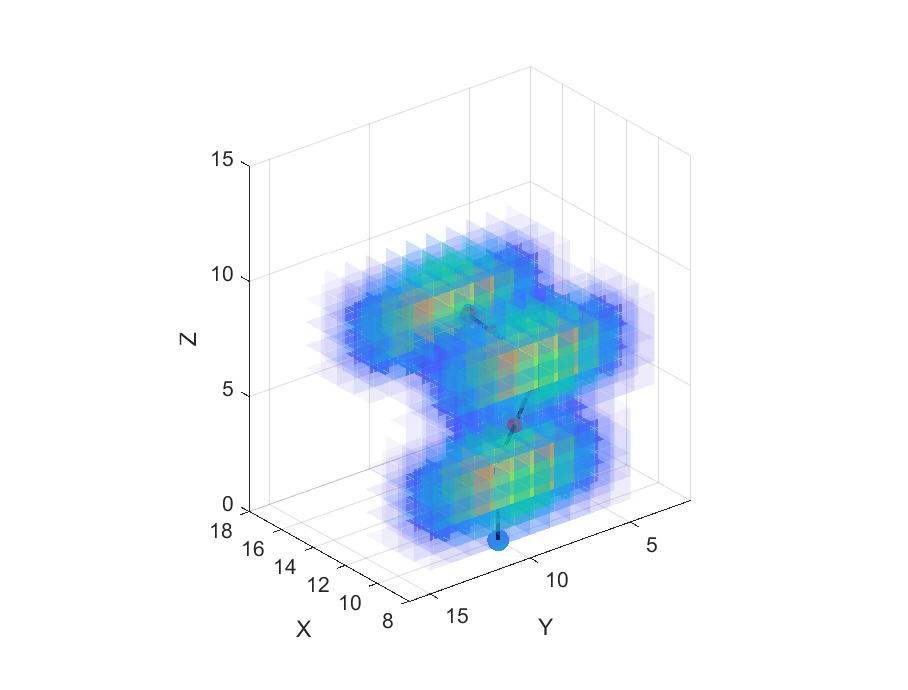
\includegraphics[width=1\textwidth]{manipulator-kernels-visualization-grid-small.eps}


\begin{equation}
	\mathrm{\vec{v}_{poi}} = 
	\begin{bmatrix}
	\sum_{(i, j, k)} W_x \odot K_x \\
	\sum_{(i, j, k)} W_y \odot K_y \\
	\sum_{(i, j, k)} W_z \odot K_z	
	\end{bmatrix}
	\label{eq:poi_velocity}
\end{equation}



 
 \add{
 	-there is an option of interpolation plot different matrixes, that are sligthely moved ... \\
 	-in results maybe compare smoothenss of interpolated and non-interpolated method
 }
 
 

\add{
	- kinematic calculations \\
	- null spaces calculations \\
	- how to join multiple velocities - weights \\
	- general overview	\\
}

***

\add{	
	- object detection is done in task domain and not c-space (more logical) \\
	- repulsive field calculation - matrix "convolution" method \\
	- matrix size and shape selection \\
	- equation for repulsive kernel values (non-linear) \\
	- PLOT: (ERK) kernel graphics \\
	- PLOT: (ERK) linear kernel graphics \\
	- PLOT: kernel field shape 	\\
	- what if there are obstacles behind wall (usually not the case, depth sensors show only thin walls, some noise doesnt matter, non-linear kernel, possible additional pre-convolution to convert obstacle grid to edges) \\
	- effecient calculation in dinamic environments, lacking prediction capabilities (MPC) \\
	- good for working in "statistical, noisy" obstacle grids
}

\subsubsection{Kernel Selection}
\label{chap:kernels}

The fundamental concept of our directional kernels lies in computing the repulsive field individually for each direction within the Cartesian coordinate system.\remove{ Our filters share a passing similarity to the Sobel  operator, a 2D convolutional filter frequently utilized in computer vision for calculating image gradients at specific points.}

Our kernels are designed as three-dimensional structures with a primary kernel axis aligned along a specific Cartesian direction, corresponding to the calculated repulsive velocity. The two secondary kernel axes are orthogonal to this primary axis. The distribution of values along the primary axis is inversely symmetric, exhibiting positive values on one side and negative values on the other, with the jump between max positive and max negative magnitude at the kernel's center. The function of the increase in magnitude along the primary axis of the kernel defines the shape of the repulsive velocity field, determining how the repulsive velocity changes as the point on the manipulator approaches an obstacle.

The length of the primary axis is critical, as it dictates the detection range for obstacles. Longer kernels can detect obstacles further away
from the robot, essentially extending the ’safety zone’ around the robot. If the primary axis is too long, it can lead to extra calculations and may cause the robot to unnecessarily avoid obstacles that aren't in its immediate path, making its movement and path planning less efficient. A kernel with a primary axis that is too short might restrict the robot's ability to maneuver, detecting obstacles potentially too late, compromising the robots capacity to avoid obstacles effectively (eq. \ref{eq: detect range}). Moreover, it is essential for the magnitudes at the kernel's periphery to be minimal, promoting a smooth increase in repulsive velocity when approaching the obstacle rather than a sudden spike.

\begin{equation}
	\label{eq: detect range}
	num_{primary} = \frac{2 \times \mathrm{range}}{\Delta \mathrm{grid}}\\
\end{equation}

%\remove{In the orthogonal axes, the magnitude of values diminishes with increasing distance from the core of the kernel, nearing zero at the edges. This gradation is vital for a smooth velocity transition when obstacles emerge in the kernels range. The peak magnitude is located at the kernel's core, along the primary axis. The polarity of the values is determined by their position relative to the primary axis. }

The length of the orthogonal axes influences the peripheral detection range for obstacles. Excessively wide kernels may generate repulsive velocities for objects that are not in the path of the robot, whereas too narrow kernels might only detect obstacles aligned directly with the Cartesian direction in the point of interest. When selecting the width and height of the kernel, we must consider the density of the neighboring points of interest on the robot, ensuring that the \replace{collective fields}{combination of kernels} adequately cover the entire manipulator's surrounding area.

\comment{}{PLOT: kernel with gaussian functions}
\comment{}{EQUATION: gaussian equations}

\add{- choice of velocity profile (gaussian, linear ... maybe could move this part to implementation / experiments) \\}
%\add{- maybe first debluring - line convolution operation (if thick walls) - however this might move wall back, which could cause crash }



\subsubsection{Interpolation of the Repulsive Velocity}

%Želimo, da je gibanje robota zvezno in ne skokovito. Da lahko to dosežemo je potrebno, da vsi hitrostni prispevki, ki vplivajo na robota prehajajo med seboj zvezno. Ker imamo mrežo ovir diskretno definirano, to ni res. Z zvišanjem resolucije polja ovir in se lahko zveznosti teoretično neskončno približamo, vendar pa imamo v realnosti običajno opravka z končno resolucijo. Da je velikost hitrosti kljub temu zvezna, ko prehajamo z točko interesa POI iz ene celice mreže ovir v drugo, uporabimo trilinearno interpolacijo, s katero za vsako od hitrosti v treh kartezičnih smeri posebaj interpoliramo hitrosti in dobimo zvezno in neskokovito linearno aproksimacijo pri prehodu med celicami. 
%
%Ko poznamo koordinate naše POI izračunamo za vsako od točk x,y in z koordinate zaokrožene navzgor in navzdol, da dobimo 8 okoliških celic. 
%
%Ko imamo poznane celice, uporabimo našo poznano konvolucijsko metodo, da izračunamo x,y in z komponento vektorja odbojne hitrosti za vsako od celic.
%
%Potem izvedemo za vsako od smeri vektorja odbojne hitrosti posebaj trilinearno interpolacijo odbojne hitrosti. Pri tem upoštevamo, da se izraučunane vrednosti odbojnih hitrosti nahajajo v centrih celic, pri interpolaciji torej zamaknemo koordinate poznanih vrenodsti za polovico resolucije mreže ovir v vsaki od smeri. Rezultat je vektor odbojne hitrosti, ki zvezno prehaja med diskretnimi vrednostmi izračunanimi v diskretnih točkah mreže ovir.
%

It is essential that the velocity contributions affecting the robot change smoothly. However, since our obstacle grid is discretely defined, achieving perfect continuity can be challenging. Increasing the resolution of the obstacle field can theoretically bring us closer to continuous behavior, but in practice, we are constrained by finite resolution. To ensure that the velocity remains continuous when transitioning from one cell of the obstacle grid to another at a point of interest (POI), we employ trilinear interpolation. \remove{This technique allows for a smooth and continuous linear approximation of velocities in all three Cartesian directions (x, y, and z) as the POI moves between cells.}

We start by scalling the coordinates of POI into the grid koordinate system, by multiplying it by grid resolution (eq.~\ref{eq:scale grid}). 

\begin{equation}
	\label{eq:scale grid}
	\vec{P} = \vec{p}_{\mathrm{POI}} \times\Delta \mathrm{grid}
\end{equation}

We get the indexes of the surrounding cells by first scaling the POI position by grid resolution and than rounding the position to the nearest lower and upper integer positions (eq.~\ref{eq:floor and ceil}).

%\begin{equation}
% X = \left[ \lfloor p_{x} \rfloor, \lceil p_{x} \rceil \right] 
%\end{equation}
%
%\begin{equation}
% Y = \left[ \lfloor p_{y} \rfloor, \lceil p_{y} \rceil \right] 
%\end{equation}
%
% \begin{equation}
% Z = \left[ \lfloor p_{z} \rfloor, \lceil p_{z} \rceil \right] 
%\end{equation}
	
	\begin{equation}
		\label{eq:floor and ceil}
		\vec{P} =
		\begin{bmatrix}
			X \\
			Y \\
			Z \\
		\end{bmatrix}
		=
		\begin{bmatrix}
			\; \lfloor \vec{p}_{\mathrm{POI}}(1) \rfloor \; \lceil \vec{p}_{\mathrm{POI}}(1) \rceil \;  \\
			\; \lfloor \vec{p}_{\mathrm{POI}}(2) \rfloor \; \lceil \vec{p}_{\mathrm{POI}}(2) \rceil \; \\
			\; \lfloor \vec{p}_{\mathrm{POI}}(3) \rfloor \; \lceil \vec{p}_{\mathrm{POI}}(3) \rceil \; 
		\end{bmatrix}
	\end{equation}

Once we got the indexes of the eight surrounding cells of our POI, we use our kernel matrix multiplication method, to calculate the 3x1 repulsive velocity vectors for all the cells (eq.~\ref{eq: calc rep vel}).

\begin{equation}
	\label{eq: calc rep vel}
	\vec{V}rep_{xyz,ijk} = \mathrm{calc\_rep\_vel}(X[i], Y[j], Z[k]) \quad \forall i, j, k \in \{1, 2\}
\end{equation}

Trilinear interpolation method works on a 3-dimensional regular grid. Before we can start with the interpolation we need to calculate the distance between POI and smaller coordinates of the cells where we calculated the repulsive velocities (eq.~\ref{eq: deltas interp}). \replace{Since the repulsive values we calculate for the cells are alligned with the centers of the cells, we need to move before the interpolation the positions of known grid points by half of the cell width.}{The calculated repulsive velocity values are located at the centers of the cells. Therefore, before interpolation, we shift the values of the cells coordinates by half the resolution of the obstacle grid for each direction. }

%\begin{equation}
%	\Delta X = \frac{\left( P_x - \left( X(1) + \frac{1}{2} \Delta \mathrm{grid} \right)  \right)}{\left( X(2) - X(1) \right)}
%\end{equation}
%
%\begin{equation}
%	\Delta Y = \frac{\left( P_y - \left( Y(1) + \frac{1}{2} \Delta \mathrm{grid} \right)  \right)}{\left( Y(2) - Y(1) \right)}
%\end{equation}
%
%\begin{equation}
%	\Delta Z = \frac{\left( P_z - \left( Z(1) + \frac{1}{2} \Delta \mathrm{grid} \right)  \right)}{\left( Z(2) - Z(1) \right)}
%\end{equation}

\begin{equation}
	\label{eq: deltas interp}
	\Delta \vec{P} =
	\begin{bmatrix}
		\Delta x \\
		\Delta y \\
		\Delta z		
	\end{bmatrix}
	=
	\begin{bmatrix}
		 \frac{\left( P_x - \left( X(1) + \frac{1}{2} \Delta \mathrm{grid} \right)  \right)}{\left( X(2) - X(1) \right)} \\
		 \frac{\left( P_y - \left( Y(1) + \frac{1}{2} \Delta \mathrm{grid} \right)  \right)}{\left( Y(2) - Y(1) \right)} \\
		 \frac{\left( P_z - \left( Z(1) + \frac{1}{2} \Delta \mathrm{grid} \right)  \right)}{\left( Z(2) - Z(1) \right)} \\
 	\end{bmatrix}
\end{equation}

The result of the interpolation is independent of the order of the operations. We first interpolate along the x-axis, followed by along the y-axis and finally along z-axis.

%\begin{equation}
%	\vec{V}_{rep,00} = \vec{V}_{rep,000}(1 - x_d) + \vec{V}_{rep,100}x_d
%\end{equation}
%\begin{equation}
%	\vec{V}_{rep,01} = \vec{V}_{rep,001}(1 - x_d) + \vec{V}_{rep,101}x_d
%\end{equation}
%\begin{equation}
%	\vec{V}_{rep,10} = \vec{V}_{rep,010}(1 - x_d) + \vec{V}_{rep,110}x_d
%\end{equation}
%\begin{equation}
%	\vec{V}_{rep,11} = \vec{V}_{rep,011}(1 - x_d) + \vec{V}_{rep,111}x_d
%\end{equation}

\begin{equation}
	\label{eq: interp x}
	\vec{V}rep_{xyz,jk} = \vec{V}rep_{xyz,0jk}(1 - \Delta x) + \vec{V}rep_{xyz,1jk} \, \Delta x \quad \forall \, j, k \in \{1, 2\}
\end{equation}

%\begin{equation}
%	\vec{V}rep_{xyz,0} = \vec{V}rep_{xyz,00}(1 - \Delta y) + \vec{V}rep_{xyz,10} \, \Delta y
%\end{equation}
%
%\begin{equation}
%	\vec{V}rep_{xyz,1} = \vec{V}rep_{xyz,01}(1 - \Delta y) + \vec{V}rep_{xyz,11} \, \Delta y
%\end{equation}

\begin{equation}
	\label{eq: interp y}
	\vec{V}rep_{xyz,k} = \vec{V}rep_{xyz,0k}(1 - \Delta y) + \vec{V}rep_{xyz,1k} \, \Delta y \quad \forall \, k \in \{1, 2\}
\end{equation}

\begin{equation}
	\label{eq: interp z}
	\vec{V}rep_{xyz} = \vec{V}rep_{xyz,0}(1 - \Delta z) + \vec{V}rep_{xyz,1} \, \Delta z 
\end{equation}

The final result is a repulsive velocity vector that transitions smoothly between the discrete values calculated at distinct points in the obstacle grid.

\comment{}{PLOT: surrounding cells, interp grid}

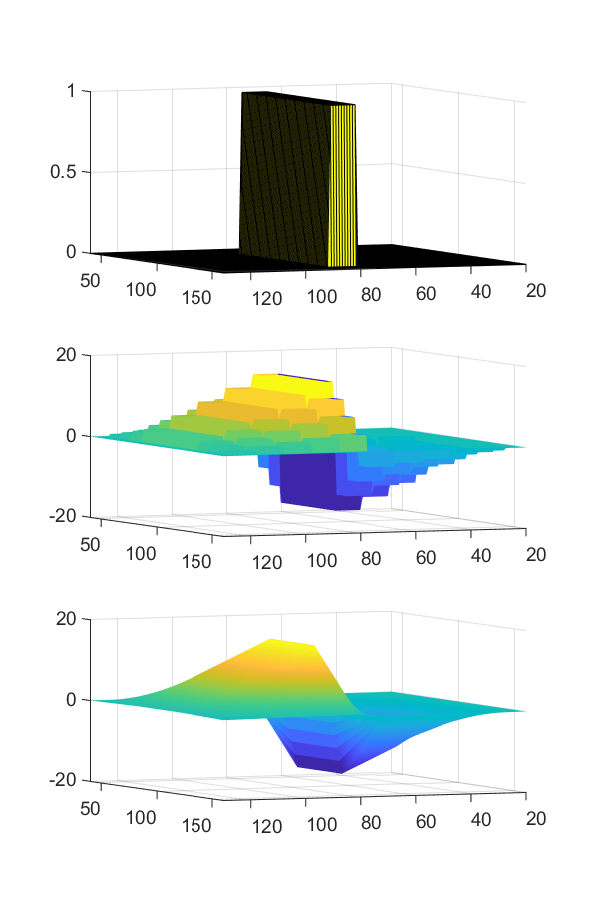
\includegraphics[width=0.75\textwidth]{field3D_visualization-3figures.eps}

\section{Implementation}

\section{Results}

\todo{3 PAGES}

\add{
	- include execution times \\
	- PLOT: kernel on robot graphics \\
	- IMPORTANT: maybe add 2D mobile platform results \\
	- use pybullet or some engine that tells you distance from obstacles and run the same task, compare distances after execution, smoothness of paths (MAYBE FOR PUBLICATION, NOT CONFERENCE)
}



\section{Discussion}

\todo{1 PAGE}

\add{
	- add the limitations of such method (already mentioned by Khatib) \\
	- the limitations of local search \\
	- good for parellelization \\
	- number of parameters that need to be tuned (are there actually that many?)
}

\section{Conclusion}



\end{document}
